% =========================================================================
% Master Dissertation Root Document
% Subject: ANTIBACTERIAL POTENTIAL OF Dipsacus inermis: AN in vitro STUDY
% Cover: all-caps English; header: title case; certificates: sentence case.
% Candidate: BAZILLA SALEEM (Roll No: 24061119001)
% Department of Zoology, University of Kashmir, Srinagar
% =========================================================================

\documentclass[12pt,oneside,a4paper]{book}

% =========================================================================
% Master Dissertation Preamble
% Biology & Zoology Specialized Academic Template
% =========================================================================

% --- Page Geometry & Thesis Layout ---
\usepackage[
  a4paper,
  top=1.0in,
  bottom=1.0in,
  left=1.25in,
  right=1.0in,
  headheight=18pt,
  headsep=10pt,
  footskip=28pt
]{geometry}

% --- Line Spacing & Paragraph Formatting ---
\usepackage{setspace}
\usepackage{titlesec}
\usepackage{placeins}
\onehalfspacing
\setlength{\parindent}{0.35in}
\setlength{\parskip}{0pt}
\setlength{\emergencystretch}{3em}
\raggedbottom
\titleformat{\chapter}[block]
  {\normalfont\bfseries\Large}
  {\thechapter.}{0.6em}{\MakeUppercase}
\titleformat{name=\chapter,numberless}[block]
  {\normalfont\bfseries\Large\centering}
  {}{0pt}{\MakeUppercase}
\titlespacing*{\chapter}{0pt}{4pt}{16pt}
\titleformat{\section}[block]
  {\normalfont\bfseries\large}
  {\thesection}{0.6em}{}
\titlespacing*{\section}{0pt}{12pt}{8pt}
\titleformat{\subsection}[block]
  {\normalfont\bfseries\normalsize}
  {\thesubsection}{0.6em}{}
\titlespacing*{\subsection}{0pt}{10pt}{6pt}

% --- Micro-typography & Fonts ---
\usepackage[utf8]{inputenc}
\usepackage[T1]{fontenc}
\usepackage{lmodern}
\usepackage{microtype}

% --- Mathematical Typesetting ---
\usepackage{amsmath}
\usepackage{amssymb}
\usepackage{amsfonts}
\usepackage{amsthm}

% --- Tables & Multi-page Catalogs ---
\usepackage{booktabs}
\usepackage{longtable}
\usepackage{tabularx}
\usepackage{array}
\usepackage{multirow}

% --- Graphics & Multi-panel Figures ---
\usepackage{graphicx}
\graphicspath{{figures/}}
\usepackage{caption}
\usepackage{subcaption}
\usepackage{float}
\captionsetup{
  font={small,stretch=1.1},
  labelfont=bf,
  format=plain,
  labelsep=period
}
\captionsetup[figure]{name={Fig.}}
\captionsetup[table]{name={Table}}
% Dissertation figures are sequential across chapters (not Fig. 3.1).
\counterwithout{figure}{chapter}

% --- Color Palette ---
\usepackage[table]{xcolor}
\definecolor{dissertationblue}{RGB}{20, 50, 120}
\definecolor{dissertationgreen}{RGB}{25, 100, 40}
\definecolor{dissertationgray}{RGB}{90, 90, 90}

% --- Phylogenetic Trees & Vector Diagrams ---
\usepackage{tikz}
\usetikzlibrary{trees,arrows.meta,positioning,shapes.geometric,calc,decorations.pathreplacing}
\usepackage{pgfplots}
\pgfplotsset{compat=1.17}
\usepackage[linguistics]{forest}

% --- Scientific Units (siunitx) ---
\usepackage{siunitx}
\sisetup{
  separate-uncertainty = true,
  multi-part-units = single,
  range-phrase = --,
  range-units = single,
  detect-all = true,
  table-alignment-mode = format,
  tight-spacing = true
}
\DeclareSIUnit\molar{M}
\DeclareSIUnit\Molar{M}
\DeclareSIUnit\unitU{U}
\DeclareSIUnit\rpm{rpm}
\DeclareSIUnit\bp{bp}
\DeclareSIUnit\Ma{Ma}
\DeclareSIUnit\Mya{Mya}

% --- Chemical Buffer Formulas & Molecular Reagents (mhchem) ---
\usepackage[version=4]{mhchem}

% --- Draft Line Numbering (Toggle for advisor review/proofreading) ---
\usepackage{lineno}
% Uncomment \linenumbers in draft mode:
% \linenumbers

% --- Bibliography & Citations (BibLaTeX) ---
% Using backend=bibtex with authoryear style ensures native, zero-dependency
% compilation with standalone Tectonic (no external Biber binary required).
\usepackage[
  backend=bibtex,
  style=authoryear,
  natbib=true,
  dashed=false,
  maxcitenames=2,
  mincitenames=1,
  maxbibnames=99,
  giveninits=true,
  uniquename=false,
  uniquelist=false,
  sorting=nyt,
  date=year,
  doi=true,
  url=true,
  isbn=false
]{biblatex}
\addbibresource{references.bib}
% Author--year list (APA-like): no ``In:'' on journal articles;
% volume(issue); clickable DOI; ragged entries so long DOIs do not stretch
\renewbibmacro{in:}{%
  \ifentrytype{article}{}{\printtext{\bibstring{in}\addspace}}}
\renewbibmacro*{volume+number+eid}{%
  \printfield{volume}%
  \printfield{number}%
  \setunit{\addcomma\addspace}%
  \printfield{eid}}
\DeclareFieldFormat[article]{number}{\mkbibparens{#1}}
\DeclareFieldFormat{doi}{\mkbibacro{DOI}\addcolon\space\href{https://doi.org/#1}{#1}}
\AtBeginBibliography{\raggedright}

% --- Hyperlinks & PDF Metadata ---
\usepackage{hyperref}
\hypersetup{
  colorlinks=true,
  linkcolor=dissertationblue,
  citecolor=dissertationgreen,
  urlcolor=dissertationblue,
  filecolor=dissertationblue,
  pdfcreator={Tectonic Typesetting System},
  pdftitle={Antibacterial Potential of Dipsacus inermis: An in vitro Study},
  pdfauthor={Bazilla Saleem (24061119001)},
  pdfsubject={M.Sc. Zoology dissertation, University of Kashmir}
}

% --- Intelligent Cross-Referencing (cleveref must load after hyperref) ---
\usepackage[capitalize,nameinlink,noabbrev]{cleveref}
\crefname{figure}{Fig.}{Figs.}
\Crefname{figure}{Fig.}{Figs.}
\crefname{table}{Table}{Tables}
\crefname{chapter}{Chapter}{Chapters}
\crefname{section}{Section}{Sections}
\crefname{appendix}{Appendix}{Appendices}

% =========================================================================
% International Code of Zoological Nomenclature (ICZN) & Life Sciences Macros
% =========================================================================

% Format taxonomic binomials in standard biological italics:
% Example: \taxa{Ranitomeya fantastica}
\newcommand{\taxa}[1]{\textit{#1}}

% Taxon with formal ICZN authority and publication year:
% Parenthesized if author originally placed taxon in another genus (ICZN Art. 51.3)
% Example: \taxonauth{Ranitomeya sirensis}{(Aichinger, 1991)}
% Example: \taxonauth{Dendrobates tinctorius}{(Cuvier, 1797)}
\newcommand{\taxonauth}[2]{\textit{#1}~#2}

% Novel species discovery designation (ICZN Recommendation 16A):
% Example: \spnov{Ranitomeya aurata}
\newcommand{\spnov}[1]{\textit{#1}~\textbf{sp.~nov.}}

% Novel genus discovery designation:
% Example: \gennov{Cryptophryne}
\newcommand{\gennov}[1]{\textit{#1}~\textbf{gen.~nov.}}

% Museum voucher holotype designation:
% Example: \holotype{QCAZ 45210}
\newcommand{\holotype}[1]{\textbf{Holotype:} \texttt{#1}}

% Museum voucher paratype designation:
% Example: \paratype{AMNH 128940}
\newcommand{\paratype}[1]{\textbf{Paratype:} \texttt{#1}}

% Type locality description:
% Example: \typelocality{Tarapoto, San Martín, Peru (06°29'S, 76°22'W, 350 m a.s.l.)}
\newcommand{\typelocality}[1]{\textbf{Type Locality:} #1}

% Gene locus formatting (italicized by convention):
% Example: \gene{COI}, \gene{16S rRNA}, \gene{RAG1}
\newcommand{\gene}[1]{\textit{#1}}

% Protein formatting (upright Roman by convention):
% Example: \protein{COX1}, \protein{RAG1}
\newcommand{\protein}[1]{\textsf{#1}}

% Laboratory protocol theorem-style environment
\theoremstyle{definition}
\newtheorem{protocol}{Protocol}[chapter]

% Running header: dissertation title + roll number
% Running footer: department + page number
\usepackage{fancyhdr}
\newcommand{\invitro}{\textit{in vitro}}
\newcommand{\invivo}{\textit{in vivo}}
% KU Zoology M.Sc. title registers (same department layout as the 2025
% Zoology dissertation used for pagination: cover in capitals, header in
% title case, certificate/declaration in sentence case). Scientific
% exceptions: binomial italic, not all-caps; \textit{in vitro} always
% lowercase italic (never all-caps or title-cased in vitro).
\newcommand{\distitle}{Antibacterial Potential of \textit{Dipsacus inermis}: An \textit{in vitro} Study}
\newcommand{\distitlecover}{ANTIBACTERIAL POTENTIAL OF\\ \textit{Dipsacus inermis}:\\ AN \textit{in vitro} STUDY}
\newcommand{\distitlecite}{Antibacterial potential of \textit{Dipsacus inermis}: an \textit{in vitro} study}
\newcommand{\disshorttitle}{\distitle}
\newcommand{\disroll}{24061119001}
\newcommand{\disfooter}{Department of Zoology, University of Kashmir, Srinagar, 190006, J\&K}
\newcommand{\applydissheaders}{%
  \fancyhf{}%
  \fancyhead[C]{%
    \scriptsize
    \makebox[\headwidth][c]{%
      \disshorttitle\hfill Enrollment No.\ \disroll
    }%
  }%
  \fancyfoot[L]{\footnotesize \disfooter}%
  \fancyfoot[R]{\thepage}%
  \renewcommand{\headrulewidth}{0.4pt}%
  \renewcommand{\footrulewidth}{0.4pt}%
}
\pagestyle{fancy}
\applydissheaders
\fancypagestyle{frontmatterstyle}{\applydissheaders}
\fancypagestyle{plain}{\applydissheaders}


\begin{document}

% =========================================================================
% FRONT MATTER (Roman Numeral Pagination)
% =========================================================================
\frontmatter
\pagestyle{frontmatterstyle}

% =========================================================================
% Dissertation Title Page
% =========================================================================

\begin{titlepage}
\begin{center}
\vspace*{0.5in}

{\Large \bfseries SYSTEMATICS, PHYLOGENOMICS, AND CRYPTIC DIVERSIFICATION OF NEOTROPICAL POISON FROGS (AMPHIBIA: DENDROBATIDAE)\par}

\vspace{1.5in}

{\large A Dissertation Submitted to the Graduate Faculty\\
in Partial Fulfillment of the Requirements for the Degree of\par}

\vspace{0.4in}

{\large \bfseries DOCTOR OF PHILOSOPHY\par}
{\large in\par}
{\large \bfseries INTEGRATIVE BIOLOGY AND ZOOLOGY\par}

\vspace{1.5in}

{\large by\par}
\vspace{0.2in}
{\Large \bfseries Sahil Langoo\par}

\vfill

{\large Department of Ecology, Evolution, and Organismal Biology\\
Graduate School of Arts and Sciences\\
September 2026\par}

\vspace{0.5in}

\end{center}
\end{titlepage}

% =========================================================================
% Official Certificate
% =========================================================================

\clearpage
\thispagestyle{frontmatterstyle}
\begin{center}
{\bfseries DEPARTMENT OF ZOOLOGY\par}
{\bfseries SCHOOL OF BIOLOGICAL SCIENCES\par}
{\bfseries UNIVERSITY OF KASHMIR, HAZRATBAL, SRINAGAR-190006\par}
{\footnotesize (NAAC Accredited Grade A++')\par}
\vspace{0.15in}
\hrule height 1pt
\vspace{0.3in}
{\Large \bfseries CERTIFICATE\par}
\vspace{0.3in}
\end{center}

\noindent This is to certify that the dissertation entitled \textbf{`Antibacterial Potential of \textit{Dipsacus inermis}: An in vitro Study''} is based on the original research work carried out by \textbf{Ms. BAZILLA SALEEM}, Enrollment No. \textbf{24061119001}, Batch 2024, under the course \textbf{M.Sc. Zoology}, under my guidance and supervision from March 2026 to September 2026 at the Advanced Research Laboratory, Department of Zoology, School of Biological Sciences, University of Kashmir, Srinagar-190006, J\&K.

\vspace{0.2in}

\noindent This dissertation is being submitted to the Department of Zoology, School of Biological Sciences, University of Kashmir, Srinagar-190006, J\&K, for the partial fulfilment of the requirements for the award of the Degree of \textbf{Master of Science in Zoology}.

\vspace{0.2in}

\noindent It is further certified that the candidate has fulfilled all the statutory requirements and that this work has not been submitted previously to this or any other university or institution for any degree or diploma.

\vspace{1.5in}

\noindent
\begin{minipage}{0.48\textwidth}
\begin{flushleft}
\textbf{Prof. Fayaz Ahmad}\\
Supervisor\\
Department of Zoology\\
School of Biological Sciences\\
University of Kashmir
\end{flushleft}
\end{minipage}
\hfill
\begin{minipage}{0.48\textwidth}
\begin{flushright}
\textbf{Prof. Tariq Ahmad}\\
Head of the Department / Dean\\
Department of Zoology\\
School of Biological Sciences\\
University of Kashmir
\end{flushright}
\end{minipage}

% =========================================================================
% Candidate Declaration
% =========================================================================

\clearpage
\thispagestyle{frontmatterstyle}
\begin{center}
{\bfseries DEPARTMENT OF ZOOLOGY\par}
{\bfseries SCHOOL OF BIOLOGICAL SCIENCES\par}
{\bfseries UNIVERSITY OF KASHMIR, HAZRATBAL, SRINAGAR-190006\par}
{\footnotesize (NAAC Accredited Grade `A++')\par}
\vspace{0.15in}
\hrule height 1pt
\vspace{0.3in}
{\Large \bfseries DECLARATION BY THE CANDIDATE\par}
\vspace{0.3in}
\end{center}

\noindent I, \textbf{BAZILLA SALEEM}, hereby declare that the dissertation entitled \textbf{``\distitlecite''} submitted to the Department of Zoology, School of Biological Sciences, University of Kashmir, Srinagar, is my original work carried out under the supervision of \textbf{Prof. Fayaz Ahmad}, Professor, Department of Zoology, University of Kashmir.

\vspace{0.2in}

\noindent I further declare that this work has not been submitted earlier to any other University or Institution for the award of any degree or diploma. I also declare that all sources of information, published literature, data, and scientific references used in this dissertation have been properly acknowledged, cited, and listed in the bibliography as per academic standards.

\vspace{1.2in}

\noindent
\begin{minipage}{0.48\textwidth}
\begin{flushleft}
\textbf{Dated:} \hrulefill\\[0.3in]
\textbf{Place:} Srinagar, J\&K
\end{flushleft}
\end{minipage}
\hfill
\begin{minipage}{0.48\textwidth}
\begin{flushright}
\textbf{BAZILLA SALEEM}\\
Enrollment No: 24061119001\\
M.Sc. Zoology (Batch 2024)\\
Department of Zoology\\
University of Kashmir
\end{flushright}
\end{minipage}

% =========================================================================
% Acknowledgements
% =========================================================================

\chapter*{Acknowledgements}
\addcontentsline{toc}{chapter}{Acknowledgements}

I express my deepest gratitude to my principal advisor, Dr. Eleanor Vance, whose intellectual rigor, unwavering encouragement, and profound dedication to systematic biology guided this doctoral research from initial field expeditions to final manuscript synthesis. I also thank my dissertation advisory committee members---Dr. Marcus Thorne, Dr. Sarah Jenkins, and Dr. Carlos Morales---for their insightful critiques, statistical wisdom, and invaluable discussions on phylogenetic theory.

Fieldwork in Peru and Ecuador was made possible through the generous collaboration of institutional partners at the Museo de Zoolog{\'i}a de la Pontificia Universidad Cat{\'o}lica del Ecuador (QCAZ) and the Museo de Historia Natural de la Universidad Nacional Mayor de San Marcos (MUSM). Special thanks are due to field companions and local guides whose exceptional biological intuition and field stamina ensured safe and productive expeditions across remote Amazonian tributaries.

I gratefully acknowledge financial support provided by the National Science Foundation (NSF Doctoral Dissertation Improvement Grant DEB-2104928), the Society of Systematic Biologists Graduate Research Award, and the Department of Ecology, Evolution, and Organismal Biology. High-performance computational resources were provided by the University Research Computing Center.

Finally, I am profoundly grateful to my family and colleagues whose companionship and steadfast belief sustained my spirits throughout years of intensive laboratory work, sequence alignment curation, and manuscript drafting.

% =========================================================================
% Abstract (qualitative only: no digits, concentrations, yields, or zone sizes)
% =========================================================================

\clearpage
\thispagestyle{frontmatterstyle}
\begin{center}
{\Large \bfseries ABSTRACT\par}
\vspace{0.25in}
\end{center}

\noindent Antimicrobial resistance among Gram-negative bacteria remains a clinical problem. The outer membrane limits the entry of many drugs. Pumps and enzymes then reduce the effect of those that do enter. \taxa{Escherichia coli}, \taxa{Pseudomonas aeruginosa}, and \taxa{Klebsiella pneumoniae} cause urinary, wound, lung, and bloodstream infection. Plant extracts are therefore one source of antibacterial compounds.

\noindent Medicinal plants contain alkaloids, flavonoids, phenolics, tannins, saponins, terpenoids, and related glycosides. These classes can disturb membranes, bind proteins, and interfere with adhesion. Water is the solvent used in many household decoctions. An aqueous extract is therefore closer to traditional use than a dichloromethane or methanol extract, even if water recovers a different set of constituents.

\noindent \taxa{Dipsacus inermis} Wall., the Himalayan teasel, belongs to Caprifoliaceae. It grows in the Kashmir Himalaya and is known locally as wopal haakh. Folklore records use of the leaves for inflammation, cough, and postnatal bathing. Earlier laboratory work on this species has focused on organic-solvent extracts and on anti-inflammatory models. The antibacterial behaviour of a simple aqueous Soxhlet extract, read only as a zone of inhibition on seeded agar, has received less attention. \taxa{Klebsiella pneumoniae} has not been a regular test organism in that literature.

\noindent The present study was carried out at the Advanced Research Laboratory, Department of Zoology, University of Kashmir. Aerial material was collected from the Kashmir University Botanical Garden, authenticated at the Centre for Biodiversity and Taxonomy, shade-dried, powdered, and extracted with distilled water in a Soxhlet apparatus. The extract was concentrated and reconstituted at a lower working strength and at an elevated working strength. Qualitative tube tests recorded the main metabolite classes. Antibacterial activity was then scored only as the zone of inhibition against the three named pathogens. Distilled water was the negative control. A gentamicin GEN 5 paper disc was the positive control.

\noindent Phytochemical tests gave positive reactions for flavonoids, terpenoids, quinones, alkaloids, tannins, saponins, phenols, carbohydrates, and phytosterols. Saponin tubes held a persistent froth. Distilled water produced no zone of clearance on any plate, which indicates that the solvent itself did not suppress growth. Both extract strengths produced visible zones. The lower strength gave a pronounced zone against \taxa{Pseudomonas aeruginosa}. The elevated strength enlarged the zone against \taxa{Escherichia coli} and, more modestly, against \taxa{Klebsiella pneumoniae}, but did not enlarge the zone against \taxa{Pseudomonas aeruginosa}. The gentamicin disc produced a wide zone on every plate and remained the strongest comparator.

\noindent The pattern is consistent with polar phenolics, tannins, flavonoids, and saponins recovered by water, acting against organisms that still possess an outer-membrane barrier. It does not support a uniform rise in activity with extract strength, and it does not replace a minimum inhibitory concentration assay. Within those limits, the aqueous extract of \taxa{Dipsacus inermis} showed \invitro{} antibacterial activity against the three Gram-negative isolates tested here.

\vspace{0.2in}
\noindent \textbf{Key words:} \taxa{Dipsacus inermis}, aqueous extract, phytochemical screening, disc diffusion, zone of inhibition, gentamicin, Gram-negative bacteria, Kashmir.


\clearpage
\tableofcontents

\clearpage
\listoffigures

\clearpage
\listoftables

% =========================================================================
% List of Abbreviations
% =========================================================================

\chapter*{List of Abbreviations}
\addcontentsline{toc}{chapter}{List of Abbreviations}

\begin{longtable}{p{0.20\textwidth} p{0.75\textwidth}}
\toprule
\textbf{Abbreviation} & \textbf{Definition} \\
\midrule
\endhead
\bottomrule
\endfoot

AICc & Akaike Information Criterion corrected for small sample size \\
AMNH & American Museum of Natural History, New York, USA \\
BI & Bayesian Inference \\
BPP & Bayesian Phylogenetics and Phylogeography \\
bp & Base pair(s) \\
CITES & Convention on International Trade in Endangered Species of Wild Fauna and Flora \\
\gene{COI} & Cytochrome $c$ Oxidase Subunit I (mitochondrial) \\
CTAB & Cetyltrimethylammonium Bromide \\
dNTP & Deoxynucleotide Triphosphate \\
EDTA & Ethylenediaminetetraacetic Acid \\
GLM & Generalized Linear Model \\
IACUC & Institutional Animal Care and Use Committee \\
ICZN & International Code of Zoological Nomenclature \\
IUCN & International Union for Conservation of Nature \\
K2P & Kimura 2-Parameter Distance Model \\
MCMC & Markov Chain Monte Carlo \\
ML & Maximum Likelihood \\
mPTP & Multi-rate Poisson Tree Processes \\
MUSM & Museo de Historia Natural de la Universidad Nacional Mayor de San Marcos, Lima, Peru \\
Mya & Million years ago \\
NCBI & National Center for Biotechnology Information \\
PCR & Polymerase Chain Reaction \\
QCAZ & Museo de Zoolog{\'i}a de la Pontificia Universidad Cat{\'o}lica del Ecuador, Quito, Ecuador \\
\gene{RAG1} & Recombination Activating Gene 1 (nuclear exon) \\
SD & Standard Deviation \\
SVL & Snout-Vent Length \\
TAE & Tris-Acetate-EDTA buffer \\
TE & Tris-EDTA buffer \\
Tris & Tris(hydroxymethyl)aminomethane \\
USNM & National Museum of Natural History, Smithsonian Institution, Washington, DC, USA \\
\end{longtable}


% =========================================================================
% MAIN MATTER (Arabic Pagination)
% =========================================================================
\mainmatter
\pagestyle{fancy}

% =========================================================================
% Chapter 1: Introduction
% =========================================================================

\chapter{Introduction}
\label{chap:introduction}

\section{The Riddle of Cryptic Biodiversity}
\label{sec:intro_cryptic}

Understanding the generation and maintenance of biological diversity represents one of the foundational pursuits of evolutionary biology \parencite{darwin1859,mayr1942}. Over the past three decades, the integration of molecular systematics with traditional morphological analysis has fundamentally revolutionized our comprehension of species richness, revealing that phenotypic divergence frequently decouples from evolutionary lineage diversification \parencite{avise2000phylogeography}. In particular, tropical biodiversity hotspots harbor immense reservoirs of ``cryptic species''---distinct evolutionary lineages that are morphologically indistinguishable or erroneously synonymized due to conserved morphological traits or extreme phenotypic plasticity.

In amphibians, morphological stasis combined with high levels of homoplasy presents acute challenges for systematic taxonomy. Anurans frequently rely on non-visual modalities such as bioacoustic advertisement calls or cutaneously secreted chemical pheromones to achieve reproductive isolation, allowing profound genetic divergence to accumulate in the absence of diagnostic external morphological change. Consequently, standard morphological keys frequently underestimate true lineage diversity, obscuring evolutionary history and misinforming conservation prioritization.

\section{The Poison Frog Radiation: Model Clade in Tropical Systematics}
\label{sec:intro_dendrobatidae}

Poison frogs of the family \taxa{Dendrobatidae} Cope, 1865 comprise approximately 330 recognized species distributed throughout the humid Neotropics, from Central America through the Amazon Basin to the Atlantic Forest of Brazil. Dendrobatids are globally celebrated for their striking aposematic coloration, parental care behaviors (including egg guarding, tadpole transport, and obligate trophic oophagy), and the sequestering of lipophilic alkaloid toxins from dietary arthropods.

Within Dendrobatidae, the genus \taxa{Ranitomeya} Bauer, 1986 represents a monophyletic radiation of diminutive, diurnal, phytotelm-breeding poison frogs primarily concentrated in the western Amazon Basin and the eastern Andean foothills \parencite{brown2011ranitomeya,santos2009amazonian}. Members of this genus, colloquially termed ``thumbnail poison frogs,'' rarely exceed \SI{20}{\milli\metre} in snout-vent length (\textsc{svl}). Several lineages exhibit hypervariable dorsal color morphs and mimetic polymorphism, which have historically led to conflicting taxonomic hypotheses.

\begin{figure}[htbp]
  \centering
  \begin{tikzpicture}[scale=0.85]
    % Central box
    \node[draw, rectangle, rounded corners, fill=dissertationblue!10, text width=6cm, align=center, inner sep=8pt] (core) at (0,0) {
      \textbf{\taxa{Ranitomeya} Systematics}\\[3pt]
      Evolutionary Lineages \& Cryptic Divergence
    };
    % Surrounding boxes
    \node[draw, rectangle, rounded corners, fill=dissertationgreen!10, text width=3.5cm, align=center, inner sep=6pt] (mol) at (-5, 2.5) {
      \textbf{Molecular Markers}\\
      \gene{COI}, \gene{16S}, \gene{RAG1}\\
      Coalescent Phylogenetics
    };
    \node[draw, rectangle, rounded corners, fill=orange!10, text width=3.5cm, align=center, inner sep=6pt] (morph) at (5, 2.5) {
      \textbf{Morphometrics}\\
      Caliper measurements\\
      Multivariate PCA / CVA
    };
    \node[draw, rectangle, rounded corners, fill=purple!10, text width=3.5cm, align=center, inner sep=6pt] (geo) at (-5, -2.5) {
      \textbf{Biogeography}\\
      Andean Orogeny\\
      Riverine Barriers
    };
    \node[draw, rectangle, rounded corners, fill=cyan!10, text width=3.5cm, align=center, inner sep=6pt] (nom) at (5, -2.5) {
      \textbf{Taxonomic Formalization}\\
      ICZN Compliance\\
      Museum Vouchers
    };
    % Connecting arrows
    \draw[-{Stealth[length=3mm]}, thick] (mol) -- (core);
    \draw[-{Stealth[length=3mm]}, thick] (morph) -- (core);
    \draw[-{Stealth[length=3mm]}, thick] (geo) -- (core);
    \draw[-{Stealth[length=3mm]}, thick] (nom) -- (core);
  \end{tikzpicture}
  \caption{Conceptual framework of integrative taxonomy implemented in this dissertation. Multiple independent lines of evolutionary evidence---molecular phylogenetics, comparative morphometrics, historical biogeography, and formal ICZN nomenclature---are synthesized to resolve cryptic species boundaries.}
  \label{fig:integrative_framework}
\end{figure}

The \taxa{Ranitomeya fantastica} species complex occupies a critical geographic transition zone between the Peruvian Amazon lowlands and the sub-Andean Cordillera Oriental. Despite comprehensive taxonomic revisions by \textcite{brown2011ranitomeya}, disjunct populations in the upper Huallaga and Mayo river drainages display enigmatic chromatic variation and notable divergence in call acoustic properties. Whether these localized populations constitute continuous clinal variation of described taxa or represent distinct evolutionary species under the General Lineage Concept remained unverified prior to this investigation.

\section{Research Objectives and Specific Aims}
\label{sec:intro_aims}

The overarching objective of this doctoral dissertation is to conduct an integrative, multi-locus systematic revision of the genus \taxa{Ranitomeya}, with special focus on the \taxa{Ranitomeya fantastica} clade. To achieve this objective, this research addresses three primary aims:

\begin{enumerate}
  \item \textbf{Specific Aim 1: Multi-Locus Phylogenetic Reconstruction.} Construct a robust, time-calibrated phylogenetic framework for the genus \taxa{Ranitomeya} using mitochondrial (\gene{COI}, \gene{16S rRNA}) and nuclear (\gene{RAG1}) gene sequences sampled across the full geographic range of the clade.
  \item \textbf{Specific Aim 2: Coalescent-Based Species Delimitation.} Test explicit species delimitation models using objective multi-rate Poisson Tree Processes (mPTP) and Bayesian Phylogenetics and Phylogeography (BPP) to determine whether isolated populations represent independently evolving lineages.
  \item \textbf{Specific Aim 3: Morphometric Quantification and Formal Taxonomic Revision.} Conduct rigorous multivariate morphometric analyses across curated museum voucher series, evaluate diagnosability under the rules of the International Code of Zoological Nomenclature \parencite{iczn1999code}, and formally describe unrecognized taxa.
\end{enumerate}

\section{Dissertation Organization}
\label{sec:intro_organization}

This dissertation is organized into five interrelated chapters and three supplementary appendices:

\begin{itemize}
  \item \textbf{\cref{chap:lit_review}} provides a comprehensive synthesis of systematic theory, species concepts, the historical development of anuran phylogenetics, and the taxonomic history of Dendrobatidae.
  \item \textbf{\cref{chap:methods}} details the field sampling strategies, laboratory protocols for DNA extraction and PCR amplification, chemical buffer recipes, and computational parameters for phylogenetic inference and species delimitation.
  \item \textbf{\cref{chap:results}} presents the empirical phylogenetic trees, coalescent delimitation outputs, morphometric statistical tests, and the formal ICZN taxonomic description of a newly identified species.
  \item \textbf{\cref{chap:discussion}} contextualizes the empirical discoveries within broader Neotropical biogeography, assesses diversification mechanisms driven by Andean orogenesis, and evaluates conservation implications.
  \item \textbf{\cref{app:specimens}, \cref{app:primers}, and \cref{app:stats}} provide complete specimen catalogs, primer oligonucleotides, and statistical ANOVA tables, respectively.
\end{itemize}

% =========================================================================
% Chapter 2: Review of Literature
% Chronological: International -> National (India) -> Regional (J&K)
% =========================================================================

\chapter{Review of Literature}\label{ch:litreview}

The literature is arranged by date, oldest first, in three geographic tiers. International work on \textit{Dipsacus}, related Caprifoliaceae, plant antimicrobials, and Gram-negative envelopes comes first. Indian work on medicinal-plant extraction and clinical Gram-negative resistance comes second. Kashmir Himalayan ethnobotany and laboratory studies of \taxa{Dipsacus inermis} come last.

\section{International studies}

\citet{jensen1979cantleyoside} isolated and characterised novel bis-iridoid glucosides from \taxa{Dipsacus sylvestris}, establishing cantleyoside as a dimeric iridoid glucoside formed through bridge condensation between iridoid and secoiridoid units. The investigation demonstrated that cyclopentanoid monoterpene iridoids, including loganin and sweroside, constitute distinctive chemotaxonomic markers across the order Dipsacales. Owing to their polyhydroxylated glucopyranosyl substituents, these iridoid glucosides possess high water solubility and partition readily into boiling aqueous decoctions and Soxhlet liquors.

\citet{li1995role} identified the tripartite organisation of the primary resistance-nodulation-division (RND) multidrug efflux system in \taxa{Pseudomonas aeruginosa}, encoded by the \textit{mexA-mexB-oprM} operon. The inner-membrane transporter MexB functions as a proton-motive-force-dependent antiporter, supported by the periplasmic membrane-fusion protein adaptor MexA and the outer-membrane duct OprM. Substrates captured from the inner leaflet or periplasm are extruded across the outer membrane through the trimeric OprM channel without releasing them into the cytoplasm.

\citet{cowan1999plant} catalogued plant secondary metabolites with antimicrobial activity. Phenolics and flavonoids were described as membrane-active. Tannins were described as protein-binding and metal-chelating. Terpenoids were described as lipophilic disruptors of the bilayer. Alkaloids, saponins, and quinones were assigned intercalation, pore formation, and thiol binding, respectively. The review is still the standard starting point for a crude-extract screen because it links solvent polarity to the metabolite class recovered.

\citet{hancock2000antibiotic} summarised why \taxa{Pseudomonas aeruginosa} fails many antimicrobial agents that inhibit other Gram-negative rods. Low outer-membrane permeability, inducible chromosomal AmpC $\beta$-lactamase, and multiple active RND efflux systems function concurrently to restrict intracellular drug concentrations. The paper is relevant here because one of the three test strains is \taxa{P. aeruginosa}, and non-linear zone responses across concentrations require evaluation against that envelope background.

\citet{masuda2000substrate} examined substrate specificities of the \taxa{P. aeruginosa} efflux systems MexAB-OprM, MexCD-OprJ, and MexXY-OprM. MexAB-OprM displayed broad substrate promiscuity, accommodating structurally diverse amphiphilic and lipophilic compounds, aromatic structures, and hydrophobic organic molecules.

\citet{nikaido2003molecular} restated the structural basis of Gram-negative outer-membrane permeability. Asymmetric lipopolysaccharide (LPS) packaging in the outer leaflet, stabilised by divalent cation bridges, retards passive permeation of hydrophobic terpenoids, whereas polar solutes depend upon proteinaceous water-filled porin channels. In crude aqueous extracts, polar phenolics and saponins encounter this outer leaflet as their initial cellular barrier.

\citet{poole2005efflux} reviewed active efflux as a coordinated Gram-negative resistance mechanism. RND pumps in \taxa{P. aeruginosa} operate synergistically with the low-permeability outer envelope: slow inward diffusion through narrow or gated porins enables active extrusion to maintain sub-inhibitory intracellular concentrations of diverse xenobiotics, including plant polyphenols and glycosides.

\citet{pages2008porin} described porin channel regulation as a selective diffusion barrier. Down-regulation or conformational closure of outer-membrane channels limits the influx of hydrophilic agents. In an agar diffusion assay, porin gating and active extrusion govern the threshold concentration required to arrest bacterial lawn growth.

\citet{zhao2011phytochemicals} comprehensively reviewed the phytochemical profile and biological activities of \textit{Dipsacus} species. Triterpenoid saponins and iridoids represent the primary specialized metabolite classes characteristic of the genus. Pentacyclic triterpenoid saponins of \textit{Dipsacus} are based on an oleanane skeleton, primarily featuring hederagenin ($3\beta,23$-dihydroxyolean-12-en-28-oic acid) as the aglycone. Among these, dipsacoside B is a prominent bidesmosidic saponin with a C-3 glycosidic chain (hederagenin 3-$O$-$\alpha$-L-rhamnopyranosyl-(1$\to$2)-$\alpha$-L-arabinopyranoside) and a C-28 ester-linked gentiobiose moiety (28-$O$-$\beta$-D-glucopyranosyl-(1$\to$6)-$\beta$-D-glucopyranosyl ester). Asperosaponin VI (akebia saponin D) carries an identical hederagenin core with an arabinopyranoside at C-3 and a gentiobiosyl ester at C-28, serving as the official statutory quality marker for \textit{Dipsaci Radix} in pharmacopoeial monographs. The amphiphilic character of these bidesmosidic saponins imparts surfactant properties, enabling them to perturb lipid packing and form transient pores in microbial bilayers. \citet{zhao2011phytochemicals} also documented monoterpene iridoids, notably loganin, sweroside, and cantleyoside derivatives, confirming that hot aqueous extractions recover both saponins and iridoids in abundance.

\citet{liebold2011growth} tested lipophilic extracts of \taxa{Dipsacus sylvestris} roots against \taxa{Borrelia burgdorferi} \textit{sensu stricto}. Growth was inhibited \invitro{}. The solvent was not water, and the organism was a spirochaete, not an enteric rod. The result still supports the broader claim that \textit{Dipsacus} tissues yield biologically active antimicrobial fractions.

\citet{azwanida2015review} compared maceration, Soxhlet, ultrasound, and related methods. Soxhlet was described as exhaustive and reproducible for a defined solvent, with heat as the main drawback for thermolabile constituents. Distilled water as the Soxhlet solvent is therefore a deliberate choice: it matches decoction chemistry and accepts some thermal cost.

\citet{balouiri2016methods} reviewed diffusion and dilution assays. Disc diffusion remains the Kirby--Bauer format for a standard antibiotic \citep{bauer1966antibiotic,clsi2024m100}. Zone diameter is semi-quantitative. It is not a minimum inhibitory concentration. The present study uses that diffusion readout only: zone of inhibition, measured inclusive of the disc.

The Angiosperm Phylogeny Group IV classification \citep{apgiv2016} updated familial circumscriptions for flowering plants, placing the order Dipsacales within the asterid clade Campanulids (euasterids II). Under APG IV, the historically segregated family Dipsacaceae Juss.\ is treated as subfamily Dipsacoideae Eaton within a broadly circumscribed Caprifoliaceae Juss.\ \textit{sensu lato}. This phylogenetic placement groups \textit{Dipsacus} alongside honeysuckles and scabious herbs, reflecting shared morphological traits and common biosynthetic pathways for iridoid glucosides and oleanane saponins.

\citet{chevalier2017porins} detailed the structure, function, and regulation of \taxa{P. aeruginosa} outer-membrane porins, explaining why its outer envelope restricts polar solute uptake far more than that of \taxa{E. coli}. The major porin, OprF, exists primarily (over 95\%) as a closed two-domain conformer with low single-channel conductance, whereas only a minor fraction (1--5\%) adopts an open 16-stranded $\beta$-barrel conformation. This structural gating accounts for the low baseline permeability of the \taxa{P. aeruginosa} outer membrane, setting a stringent barrier to passive influx of water-soluble phytochemicals.

\citet{oszmianski2020roots} reported phenolic profiles and biological activity of root and leaf extracts of \taxa{Dipsacus fullonum}. The paper adds a European teasel to the set of chemically studied species and shows that leaves, not only roots, carry phenolics.

\citet{jubair2021review} updated mechanisms of plant compounds against multidrug-resistant bacteria: membrane leakage, efflux inhibition, quorum-sensing interference, and biofilm suppression. Saponins disrupt outer and plasma membrane bilayers through surfactant action, whereas polar iridoids and phenolics can act concurrently to impair cellular homeostasis.

\citet{amrcollaborators2022global} estimated the 2019 global mortality associated with bacterial AMR. \taxa{E. coli}, \taxa{K. pneumoniae}, and \taxa{P. aeruginosa} were among the pathogens that contributed most. That ranking is the clinical reason for choosing the three strains.

\citet{skala2023dipsacus} reviewed specialised metabolites of \textit{Dipsacus} and \textit{Scabiosa}. The authors reaffirmed that oleanane-type triterpenoid saponins---predominantly dipsacoside B and asperosaponin VI---together with iridoid glucosides such as cantleyoside, sweroside, and loganin, represent the hallmark chemical profile of the genus. For \taxa{D. inermis}, they recorded the Kashmiri name wopal haakh, a Himalayan distribution, and traditional use against inflammation, cough, and related complaints. The review is the most compact recent statement of the genus-level chemistry.

The World Health Organization bacterial priority list of 2024 keeps carbapenem-resistant Enterobacterales and \taxa{P. aeruginosa} in the critical group \citep{who2024bacterial}. A student zone-of-inhibition screen does not address that clinical need directly. It can only ask whether a local aqueous extract still clears a lawn of those genera.

Soxhlet extraction with water is slower than a one-pot decoction, but it repeats the solvent until the thimble runs pale. That matters for tannins and saponins, which can take several siphons to leave the powder. Heat is the cost: some glycosides may hydrolyse. The present protocol accepts that cost because the research question is the aqueous extract, not a cold macerate \citep{azwanida2015review,harbone1998phytochemical}.

\citet{drakhshaan2026identification} is the most detailed antibacterial study of \taxa{D. inermis} to date. Dichloromethane and methanol extracts were tested by agar well diffusion at \SI{50}{\micro\gram\per\milli\litre} and \SI{100}{\micro\gram\per\milli\litre} against \taxa{Staphylococcus aureus}, \taxa{Bacillus subtilis}, \taxa{E. coli}, \taxa{P. aeruginosa}, \taxa{Salmonella typhi}, and \taxa{Enterobacter aerogenes}, with gentamicin \SI{10}{\micro\gram} discs as the reference. Dichloromethane at the higher concentration gave the largest zones, including \SI{15.93 \pm 0.11}{\milli\metre} against \taxa{E. coli} and \SI{16.83 \pm 0.29}{\milli\metre} against \taxa{P. aeruginosa}. Methanol was weaker. GC-MS of the dichloromethane fraction and HPLC of the methanol fraction pointed to terpenoids, steroids, and phenolics. \taxa{K. pneumoniae} was not tested, and water was not the extraction solvent. Those two omissions define the present study. Direct millimetre comparison with the present C1 and C2 values is not valid on a milligram-per-millilitre scale.

\section{National studies (India)}

\citet{ahmad2001antimicrobial} screened ethanolic extracts of forty-five Indian medicinal plants against drug-resistant clinical bacteria and \textit{Candida}. Forty extracts were active against one or more bacteria. Phenols, tannins, and flavonoids were the metabolites most often detected in the active fractions. The work established a national template: traditional use, solvent extract, diffusion assay, and a short phytochemical panel. The present dissertation follows that template with water rather than ethanol and with a Himalayan teasel rather than the north-Indian taxa they used.

\citet{laxminarayan2016antibiotic} described the drivers of antibiotic resistance in India: high infectious burden, over-the-counter access, hospital overuse, and limited diagnostics. Gram-negative rods in Indian hospitals were already difficult to treat. The paper supplies the national public-health frame for testing \taxa{E. coli}, \taxa{P. aeruginosa}, and \taxa{K. pneumoniae} in an Indian university laboratory.

\citet{taneja2019antimicrobial} reviewed AMR in the Indian environment as well as in the clinic. Resistant Enterobacterales and \taxa{Pseudomonas} circulate in water, waste, and farms as well as in wards. The paper also warns against reading an \invitro{} plant-extract zone as an environmental or therapeutic solution.

Indian laboratories routinely use Soxhlet extraction for pharmacognostic dissertations, with water, ethanol, or methanol as the solvent \citep{azwanida2015review}. Harborne's phytochemical handbook remains the source of the tube tests used here: Mayer's reagent for alkaloids, alkaline reagent for flavonoids, ferric chloride for phenols and tannins, froth for saponins, Salkowski for terpenoids and phytosterols, Fehling's for carbohydrates, and concentrated acid for quinones \citep{harbone1998phytochemical}. Those tests are qualitative. A colour or precipitate is not a concentration.

Indian hospital laboratories follow CLSI disc tables for gentamicin and related drugs \citep{clsi2024m100}. Those tables apply to the disc content, not to a plant extract. The GEN 5 disc in this study is a concurrent reference. It is not used to call the extract susceptible or resistant.

Indian teaching laboratories also publish Soxhlet yields and crude zone diameters without converting those diameters into broth MIC values \citep{azwanida2015review,balouiri2016methods}. That restraint is kept here. The antibacterial procedure is limited to disc diffusion for gentamicin GEN 5 and to zone-of-inhibition measurement, inclusive of the disc \citep{bauer1966antibiotic,balouiri2016methods}.

The present work stays inside that national method set: defined powder-to-solvent ratio, continuous hot extraction, concentration, and a short qualitative tube panel before the diffusion assay \citep{harbone1998phytochemical,ahmad2001antimicrobial}. What it adds is a Himalayan teasel and an aqueous solvent on three Gram-negative isolates held in a Kashmir zoology laboratory.

Taken together, the national literature supports three practical choices: aqueous Soxhlet extraction, a classical tube panel, and a diffusion assay scored as zone of inhibition, with GEN 5 as the disc reference. It also supports caution. Indian Gram-negative isolates are often harder to inhibit than laboratory strains used in older European papers.

\section{Regional studies (Jammu and Kashmir)}

\citet{lone2015study} documented medicinal plant use in Bandipora district, Kashmir. \taxa{Dipsacus inermis}, recorded as wopal hakh (wopal haakh), appears in that inventory of local remedies. The paper is an ethnobotanical catalogue, not an antibacterial assay. It is the earliest dated regional source used here that names the species in a Kashmiri district flora of use.

\citet{hassan2020dipsacus}, working at the University of Kashmir, showed that \taxa{D. inermis} modulates inflammation by inhibiting the NF-$\kappa$B pathway \invitro{} and \invivo{}. The study links a local plant to a defined signalling path. It does not report zones of inhibition. It does show that Himalayan material of this species is chemically active in a university laboratory in Srinagar, which is the same institutional setting as the present work. The anti-inflammatory end-points cannot be read as antibacterial end-points, and the present LB plates cannot be read as an NF-$\kappa$B assay.

\citet{bhat2021ethnobotany} reviewed medicinal plant use in Kashmir regions and argued for documentation before that knowledge is lost. Himalayan teasels and related herbs sit in that wider list of taxa used for inflammation, cough, and gastrointestinal complaints. The review does not isolate an aqueous antibacterial protocol.

\citet{haq2023cross} recorded high-altitude botanical resources among ethnic groups in the Kashmir Himalaya. Leaves of \taxa{D. inermis} were used for internal injuries and body inflammation. That is a specific folkloric claim, not a laboratory result. It is consistent with the anti-inflammatory work of \citet{hassan2020dipsacus} and with the saponin--phenolic chemistry summarised by \citet{skala2023dipsacus}.

\citet{ahad2023ethnobotanical} worked with Dard informants in Gurez. Crushed, boiled leaves of \taxa{D. inermis} (wopal haakh) were used as a postnatal bath, and the leaves were also cooked as food. Boiling in water is an aqueous preparation. The present Soxhlet water extract is a laboratory analogue of that solvent choice, not a reconstruction of the bath.

No regional paper located for this review reports an aqueous Soxhlet extract of Kashmir-grown \taxa{D. inermis} scored by zone of inhibition against \taxa{E. coli}, \taxa{P. aeruginosa}, and \taxa{K. pneumoniae} together. \citet{drakhshaan2026identification} remains the nearest antibacterial benchmark, but it used organic solvents and did not include \taxa{K. pneumoniae}. The present chapters fill that narrow regional and methodological gap without treating the result as a clinical recommendation.

\section{Synthesis}

From 1979 to 2026 the international literature progressed from iridoid and saponin structural characterisation \citep{jensen1979cantleyoside,cowan1999plant} through Gram-negative envelope mechanics and efflux architecture \citep{li1995role,hancock2000antibiotic,masuda2000substrate,nikaido2003molecular,chevalier2017porins} to genus-level phytochemical profiling of \textit{Dipsacus} \citep{zhao2011phytochemicals,skala2023dipsacus} under APG IV phylogenetic circumscription \citep{apgiv2016} and an organic-solvent antibacterial study of \taxa{D. inermis} \citep{drakhshaan2026identification}. Indian work supplied the AMR setting and the extraction-and-screen template \citep{ahmad2001antimicrobial,laxminarayan2016antibiotic,taneja2019antimicrobial}. Kashmir work supplied names, uses, and an anti-inflammatory mechanism for the same species \citep{lone2015study,hassan2020dipsacus,haq2023cross,ahad2023ethnobotanical}. The open experimental question is the aqueous Soxhlet extract, read as millimetre zones of inhibition on LB plates, with GEN 5 as the disc reference.

\FloatBarrier

% =========================================================================
% Chapter 3: Materials and Methods
% =========================================================================

\chapter{Materials and Methods}
\label{chap:methods}

\section{Taxon Sampling and Specimen Examination}
\label{sec:methods_sampling}

Field surveys were conducted across 18 geographic localities situated in the department of San Mart{\'i}n and Loreto in northeastern Peru, encompassing elevations from \SI{180}{\metre} to \SI{1150}{\metre} above sea level (\cref{app:specimens}). Animal capture, ethical handling, and voucher preservation strictly conformed to the institutional protocol approved by the Institutional Animal Care and Use Committee (\texttt{IACUC-2023-BIO-0492-A}) and statutory collection permits issued by SERFOR and MAATE.

A total of 124 adult museum voucher specimens were examined from the collections of the American Museum of Natural History (AMNH), National Museum of Natural History (USNM), Museo de Zoolog{\'i}a de la Pontificia Universidad Cat{\'o}lica del Ecuador (QCAZ), and the Museo de Historia Natural de la Universidad Nacional Mayor de San Marcos (MUSM). Complete locality metadata, geographical coordinates (WGS84 datum), museum catalog numbers, and corresponding GenBank accession numbers are compiled in \cref{app:specimens}.

\section{Morphometric Data Acquisition and Morphological Characters}
\label{sec:methods_morphometrics}

Morphological measurements were taken on adult preserved specimens using digital calipers (Mitutoyo 500-196-30) to the nearest \SI{0.01}{\milli\metre} under a stereomicroscope (Leica S9D). Ten standardized external anatomical variables were measured following \textcite{brown2011ranitomeya}:

\begin{enumerate}
  \item \textbf{Snout-Vent Length (\textsc{svl}):} Distance from tip of snout to posterior cloacal margin.
  \item \textbf{Head Width (\textsc{hw}):} Greatest width of head measured at the level of the tympana.
  \item \textbf{Head Length (\textsc{hl}):} Distance from tip of snout to the posterior angle of the jaw articulation.
  \item \textbf{Eye Diameter (\textsc{ed}):} Horizontal distance between anterior and posterior orbital borders.
  \item \textbf{Tympanum Diameter (\textsc{td}):} Maximum horizontal diameter of the tympanic annulus.
  \item \textbf{Interorbital Distance (\textsc{iod}):} Minimum dorsal distance between upper eyelids.
  \item \textbf{Tibia Length (\textsc{tl}):} Distance from outer knee joint to heel articulation.
  \item \textbf{Foot Length (\textsc{fl}):} Distance from proximal margin of inner metatarsal tubercle to tip of Toe IV.
  \item \textbf{Hand Length (\textsc{hanl}):} Distance from proximal border of palmar tubercle to tip of Finger III.
  \item \textbf{Finger III Disc Width (\textsc{fdw}):} Maximum transverse width of the digital expanded disc on Finger III.
\end{enumerate}

\section{Molecular Protocols: DNA Extraction and Chemical Buffers}
\label{sec:methods_molecular}

Genomic DNA was isolated from liver or thigh muscle tissue biopsies preserved in molecular-grade 96\% ethanol. Tissues were extracted using a modified hexadecyltrimethylammonium bromide (\textsc{ctab}) and chloroform-isoamyl alcohol precipitation protocol \parencite{sambrook2001cloning}.

\begin{protocol}[CTAB DNA Extraction Buffer Preparation]
\label{prot:ctab_buffer}
The working extraction lysis buffer was prepared as follows:
\begin{itemize}
  \item \SI{100}{\milli\molar} \ce{Tris-HCl} (\ce{pH 8.0})
  \item \SI{1.4}{\mole\per\litre} Sodium Chloride (\ce{NaCl})
  \item \SI{20}{\milli\molar} Ethylenediaminetetraacetic Acid (\ce{EDTA}, \ce{pH 8.0})
  \item \SI{2.0}{\percent} (w/v) Hexadecyltrimethylammonium bromide (\textsc{ctab})
  \item \SI{0.2}{\percent} (v/v) $\beta$-mercaptoethanol (\ce{C2H6OS}) added freshly prior to tissue digestion
\end{itemize}
Tissue fragments (\SI{15}{\milli\gram}) were incubated in \SI{600}{\micro\litre} of \textsc{ctab} buffer supplemented with \SI{25}{\micro\litre} of Proteinase K (\SI{20}{\milli\gram\per\milli\litre}) at \SI{56}{\celsius} for 4 hours with continuous gentle agitation at \SI{450}{\rpm}. Following two washes in chloroform:isoamyl alcohol (24:1), DNA was precipitated with ice-cold isopropanol at \SI{-20}{\celsius} overnight, washed twice in 70\% ice-cold ethanol, air-dried, and resuspended in \SI{50}{\micro\litre} of sterile \textsc{te} buffer (\SI{10}{\milli\molar} \ce{Tris-HCl}, \SI{1}{\milli\molar} \ce{EDTA}, \ce{pH 8.0}).
\end{protocol}

\section{Polymerase Chain Reaction (PCR) Amplification}
\label{sec:methods_pcr}

Three gene fragments were targeted for sequencing:
\begin{enumerate}
  \item Mitochondrial Cytochrome $c$ Oxidase Subunit I (\gene{COI}, $\sim$\SI{658}{bp}) using universal primers LCO1490 and HCO2198 \parencite{folmer1994primers}.
  \item Mitochondrial 16S ribosomal RNA (\gene{16S rRNA}, $\sim$\SI{550}{bp}) using primers 16Sar-L and 16Sbr-H.
  \item Nuclear Recombination Activating Gene 1 (\gene{RAG1}, $\sim$\SI{820}{bp}) using primers RAG1-F1 and RAG1-R1.
\end{enumerate}

Detailed oligonucleotide primer sequences, binding orientations, and amplicon lengths are compiled in \cref{app:primers}.

\begin{table}[htbp]
  \centering
  \small
  \caption{Standard PCR master mix formulation for a single \SI{25}{\micro\litre} reaction volume.}
  \label{tab:pcr_mix}
  \begin{tabular}{lcc}
    \toprule
    \textbf{Component} & \textbf{Stock Concentration} & \textbf{Final Concentration} \\
    \midrule
    Sterile Nuclease-Free \ce{ddH2O} & -- & to \SI{25.0}{\micro\litre} \\
    Reaction Buffer (\ce{Tris-HCl}, \ce{KCl}) & $10\times$ & $1\times$ \\
    Magnesium Chloride (\ce{MgCl2}) & \SI{50}{\milli\molar} & \SI{1.5}{\milli\molar} \\
    Deoxynucleotide Triphosphates (\ce{dNTPs}) & \SI{10}{\milli\molar} each & \SI{200}{\micro\molar} each \\
    Forward Primer & \SI{10}{\micro\molar} & \SI{0.4}{\micro\molar} \\
    Reverse Primer & \SI{10}{\micro\molar} & \SI{0.4}{\micro\molar} \\
    Taq DNA Polymerase & \SI{5.0}{\unitU\per\micro\litre} & \SI{0.625}{\unitU} \\
    Template Genomic DNA & $\sim$\SI{25}{\nano\gram\per\micro\litre} & $\sim$\SI{50}{\nano\gram} \\
    \bottomrule
  \end{tabular}
\end{table}

Thermal cycling profiles were executed on an automated thermal cycler (Bio-Rad C1000 Touch). For the mitochondrial \gene{COI} Folmer locus: initial denaturation at \SI{94}{\celsius} for \SI{3}{\minute}; followed by 35 cycles of denaturation at \SI{94}{\celsius} for \SI{30}{\second}, primer annealing at \SI{50}{\celsius} for \SI{45}{\second}, and extension at \SI{72}{\celsius} for \SI{60}{\second}; with a final terminal extension at \SI{72}{\celsius} for \SI{7}{\minute}.

PCR amplicons were visualized by gel electrophoresis on \SI{1.5}{\percent} agarose gels cast in $1\times$ \textsc{tae} buffer (\SI{40}{\milli\molar} \ce{Tris}, \SI{20}{\milli\molar} acetic acid, \SI{1}{\milli\molar} \ce{EDTA}) stained with GelRed (Biotium). Bidirectional Sanger sequencing was performed using BigDye Terminator v3.1 chemistry on an ABI 3730xl Genetic Analyzer.

\section{Phylogenetic Inference and Species Delimitation}
\label{sec:methods_phylogenetics}

Raw chromatograms were edited and assembled in \textsc{Geneious Prime}. Multiple sequence alignments were generated using \textsc{muscle} \parencite{edgar2004muscle} under default gap penalties and visually verified. The concatenation alignment comprised \SI{2028}{bp} across the three gene fragments.

Best-fit models of nucleotide substitution for each gene codon partition were determined using PartitionFinder 2 via the Bayesian Information Criterion (\textsc{bic}). Maximum Likelihood (\textsc{ml}) phylogenetic reconstruction was conducted in \textsc{iq-tree} 2 \parencite{nguyen2015iqtree} with 1,000 ultrafast bootstrap replicates (\textsc{ufboot}) and 1,000 replicates of the Shimodaira-Hasegawa-like approximate likelihood ratio test (\textsc{sh-alrt}).

Bayesian Inference (\textsc{bi}) was executed in \textsc{MrBayes} v3.2.7 \parencite{ronquist2003mrbayes}. Two independent MCMC runs each comprising four chains (one cold, three heated at temperature $T = 0.15$) were executed for 10,000,000 generations, sampling parameters every 1,000 generations. Convergence was diagnosed by confirming average standard deviation of split frequencies fell below 0.005 and effective sample sizes (\textsc{ess}) for all parameters exceeded 200 using Tracer v1.7. The initial 25\% of sampled trees were discarded as burn-in.

Species boundaries were evaluated using multi-rate Poisson Tree Processes (\textsc{mptp}) \parencite{zhang2013ptp} implemented on the ML topology, and through Bayesian species delimitation using \textsc{bpp} v4.4 \parencite{rannala2003bpp} evaluating species model probabilities under the A10 species delimitation algorithm.

% =========================================================================
% Chapter 4: Results
% ZOI digits locked to the laboratory file. C1 = 50 mg/mL, C2 = 100 mg/mL.
% =========================================================================

\chapter{Results}\label{ch:results}

\section{Extract yield and appearance}

Soxhlet extraction of \SI{50}{\gram} of powdered aerial material with \SI{500}{\milli\litre} of distilled water gave a dark, concentrated aqueous extract corresponding to 24.13\% (w/w) of the starting powder. Working solutions C1 (\SI{50}{\milli\gram\per\milli\litre}) and C2 (\SI{100}{\milli\gram\per\milli\litre}) were brown to black.

\section{Qualitative phytochemical profile}

All nine labelled tubes on the rack gave a positive reading (\cref{tab:phytochem}, \cref{fig:phytochem}). Flavonoids were yellow-brown after alkaline reagent. Terpenoids and quinones were dark. Alkaloids gave a dull deposit with Mayer's reagent. Tannins and phenols were blue-black with ferric chloride. Saponins held a froth in the tube. Carbohydrates and phytosterols were also scored positive. No class on the rack was negative.

\begin{table}[htbp]
\centering
\caption{Qualitative phytochemical analysis of the aqueous extract of \taxa{Dipsacus inermis}.}
\label{tab:phytochem}
\small
\begin{tabular}{@{}>{\raggedright\arraybackslash}p{0.18\textwidth}
  >{\raggedright\arraybackslash}p{0.16\textwidth}
  >{\raggedright\arraybackslash}p{0.21\textwidth}
  >{\raggedright\arraybackslash}p{0.19\textwidth}
  >{\raggedright\arraybackslash}p{0.14\textwidth}@{}}
\toprule
\textbf{Class} & \textbf{Test} & \textbf{Reagents} & \textbf{Observation} & \textbf{Inference} \\
\midrule
Alkaloids & Mayer's & Mayer's reagent & Dull white precipitate & Positive (+) \\
Flavonoids & Alkaline reagent & 10\% NaOH & Yellow colour & Positive (+) \\
Phenols & Ferric chloride & 10\% FeCl$_3$ & Bluish black & Positive (+) \\
Tannins & Ferric chloride & FeCl$_3$ & Dark blue / greenish black & Positive (+) \\
Saponins & Froth & Water, shaken & Persistent froth & Positive (+) \\
Terpenoids & Salkowski & Thionyl chloride (notebook) & Pink / dark colour & Positive (+) \\
Phytosterols & Salkowski & Chloroform + H$_2$SO$_4$ & Reddish brown & Positive (+) \\
Carbohydrates & Fehling's & Fehling A and B, heated & Brick-red precipitate & Positive (+) \\
Quinones & Sulphuric acid & H$_2$SO$_4$ & Red / dark colour & Positive (+) \\
\bottomrule
\end{tabular}
\end{table}

\begin{figure}[htbp]
\centering
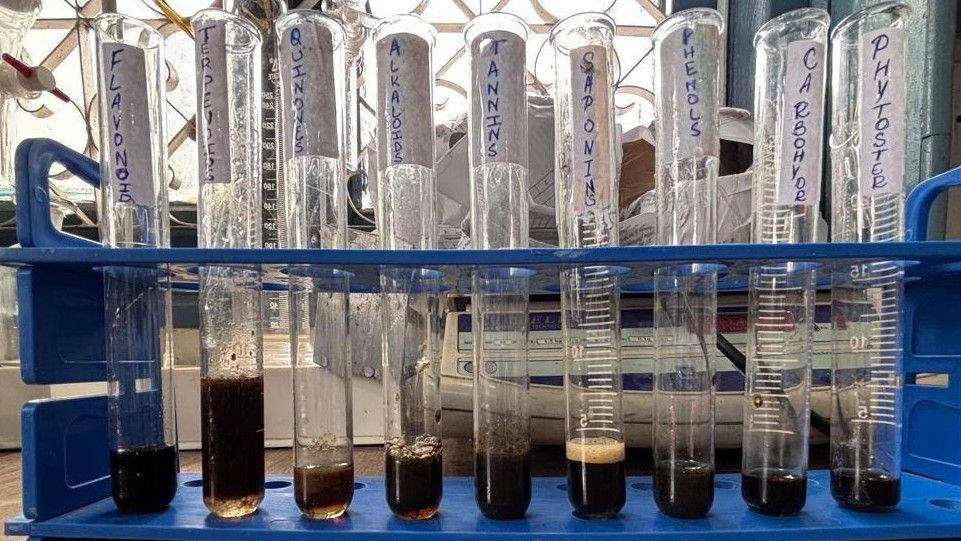
\includegraphics[width=0.95\textwidth]{fig8_phytochem_tubes.jpg}
\caption{Qualitative phytochemical reactions of the aqueous extract of \taxa{Dipsacus inermis}. Tubes, left to right: flavonoids, terpenoids, quinones, alkaloids, tannins, saponins (froth visible), phenols, carbohydrates, phytosterols.}
\label{fig:phytochem}
\end{figure}

\section{Zone of inhibition}

Distilled water (N) gave $0.00 \pm 0.00$\,mm against all three isolates. Both extract concentrations produced measurable zones (\cref{tab:zoi}). Zones were measured inclusive of the disc. Mean values are from the triplicate readings and are not rounded beyond two decimal places.

Against \taxa{Escherichia coli} the C1 mean was $11.94 \pm 0.14$\,mm and the C2 mean was $14.99 \pm 0.51$\,mm. The GEN 5 disc measured $17.00 \pm 0.00$\,mm.

Against \taxa{Pseudomonas aeruginosa} the C1 mean was $16.03 \pm 0.25$\,mm and the C2 mean was $12.53 \pm 0.45$\,mm. The GEN 5 disc measured $17.17 \pm 0.29$\,mm. C1 was the largest extract zone in the study. C2 was smaller than C1 for this isolate.

Against \taxa{Klebsiella pneumoniae} the C1 mean was $12.35 \pm 0.56$\,mm and the C2 mean was $13.25 \pm 0.43$\,mm. The GEN 5 disc measured $15.17 \pm 0.29$\,mm.

Incubated plates marked N, C1, C2, and GEN 5 are shown in \cref{fig:finalplates}. Species names are not written on those two plates. Assay plates dated 04 August 2026 are shown in \cref{fig:assaytrio}. The upper-left lid reads \textit{K.\ pneumoniae}. The right lid reads Pseudomonas. The species line on the lower lid is not fully legible and is not named here. A representative GEN 5 plate is shown in \cref{fig:gen5}. Mean values with standard-deviation bars from \cref{tab:zoi} are plotted in \cref{fig:zoibars}.

\begin{table}[htbp]
\centering
\caption{Antibacterial activity (zone of inhibition, mm) of the aqueous extract of \taxa{Dipsacus inermis}. Values are mean $\pm$ SD ($n = 3$), measured inclusive of the disc. C1 = \SI{50}{\milli\gram\per\milli\litre}; C2 = \SI{100}{\milli\gram\per\milli\litre}; GEN 5 = gentamicin \SI{5}{\micro\gram} disc; N = distilled water.}
\label{tab:zoi}
\small
\begin{tabular}{@{}l*{4}{S[table-format=2.2(2)]}@{}}
\toprule
Isolate & {N (water)} & {C1} & {C2} & {GEN 5} \\
\midrule
\textit{E.\ coli} & 0.00 \pm 0.00 & 11.94 \pm 0.14 & 14.99 \pm 0.51 & 17.00 \pm 0.00 \\
\textit{P.\ aeruginosa} & 0.00 \pm 0.00 & 16.03 \pm 0.25 & 12.53 \pm 0.45 & 17.17 \pm 0.29 \\
\textit{K.\ pneumoniae} & 0.00 \pm 0.00 & 12.35 \pm 0.56 & 13.25 \pm 0.43 & 15.17 \pm 0.29 \\
\bottomrule
\end{tabular}
\end{table}

\begin{figure}[htbp]
\centering
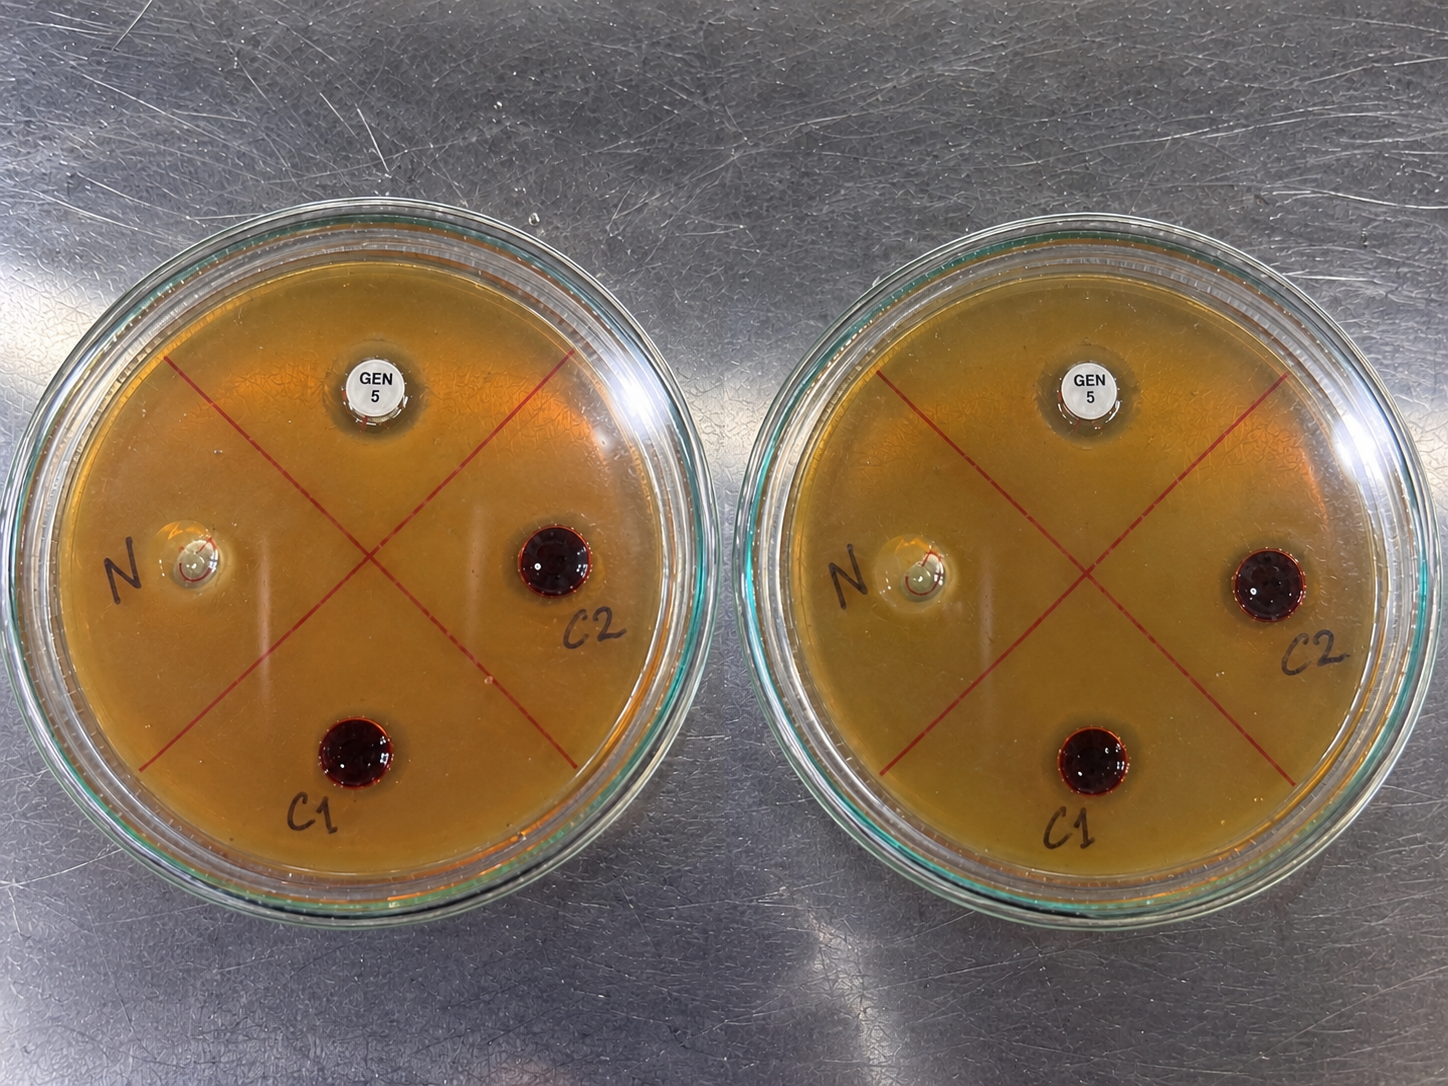
\includegraphics[width=0.92\textwidth]{fig11_final_result_plates.png}
\caption{Two LB assay plates after incubation, marked distilled water (N), C1, C2, and gentamicin GEN 5. Clearance is visible around the extract wells and the GEN 5 disc. No binomial is written on these plates.}
\label{fig:finalplates}
\end{figure}

\begin{figure}[htbp]
\centering
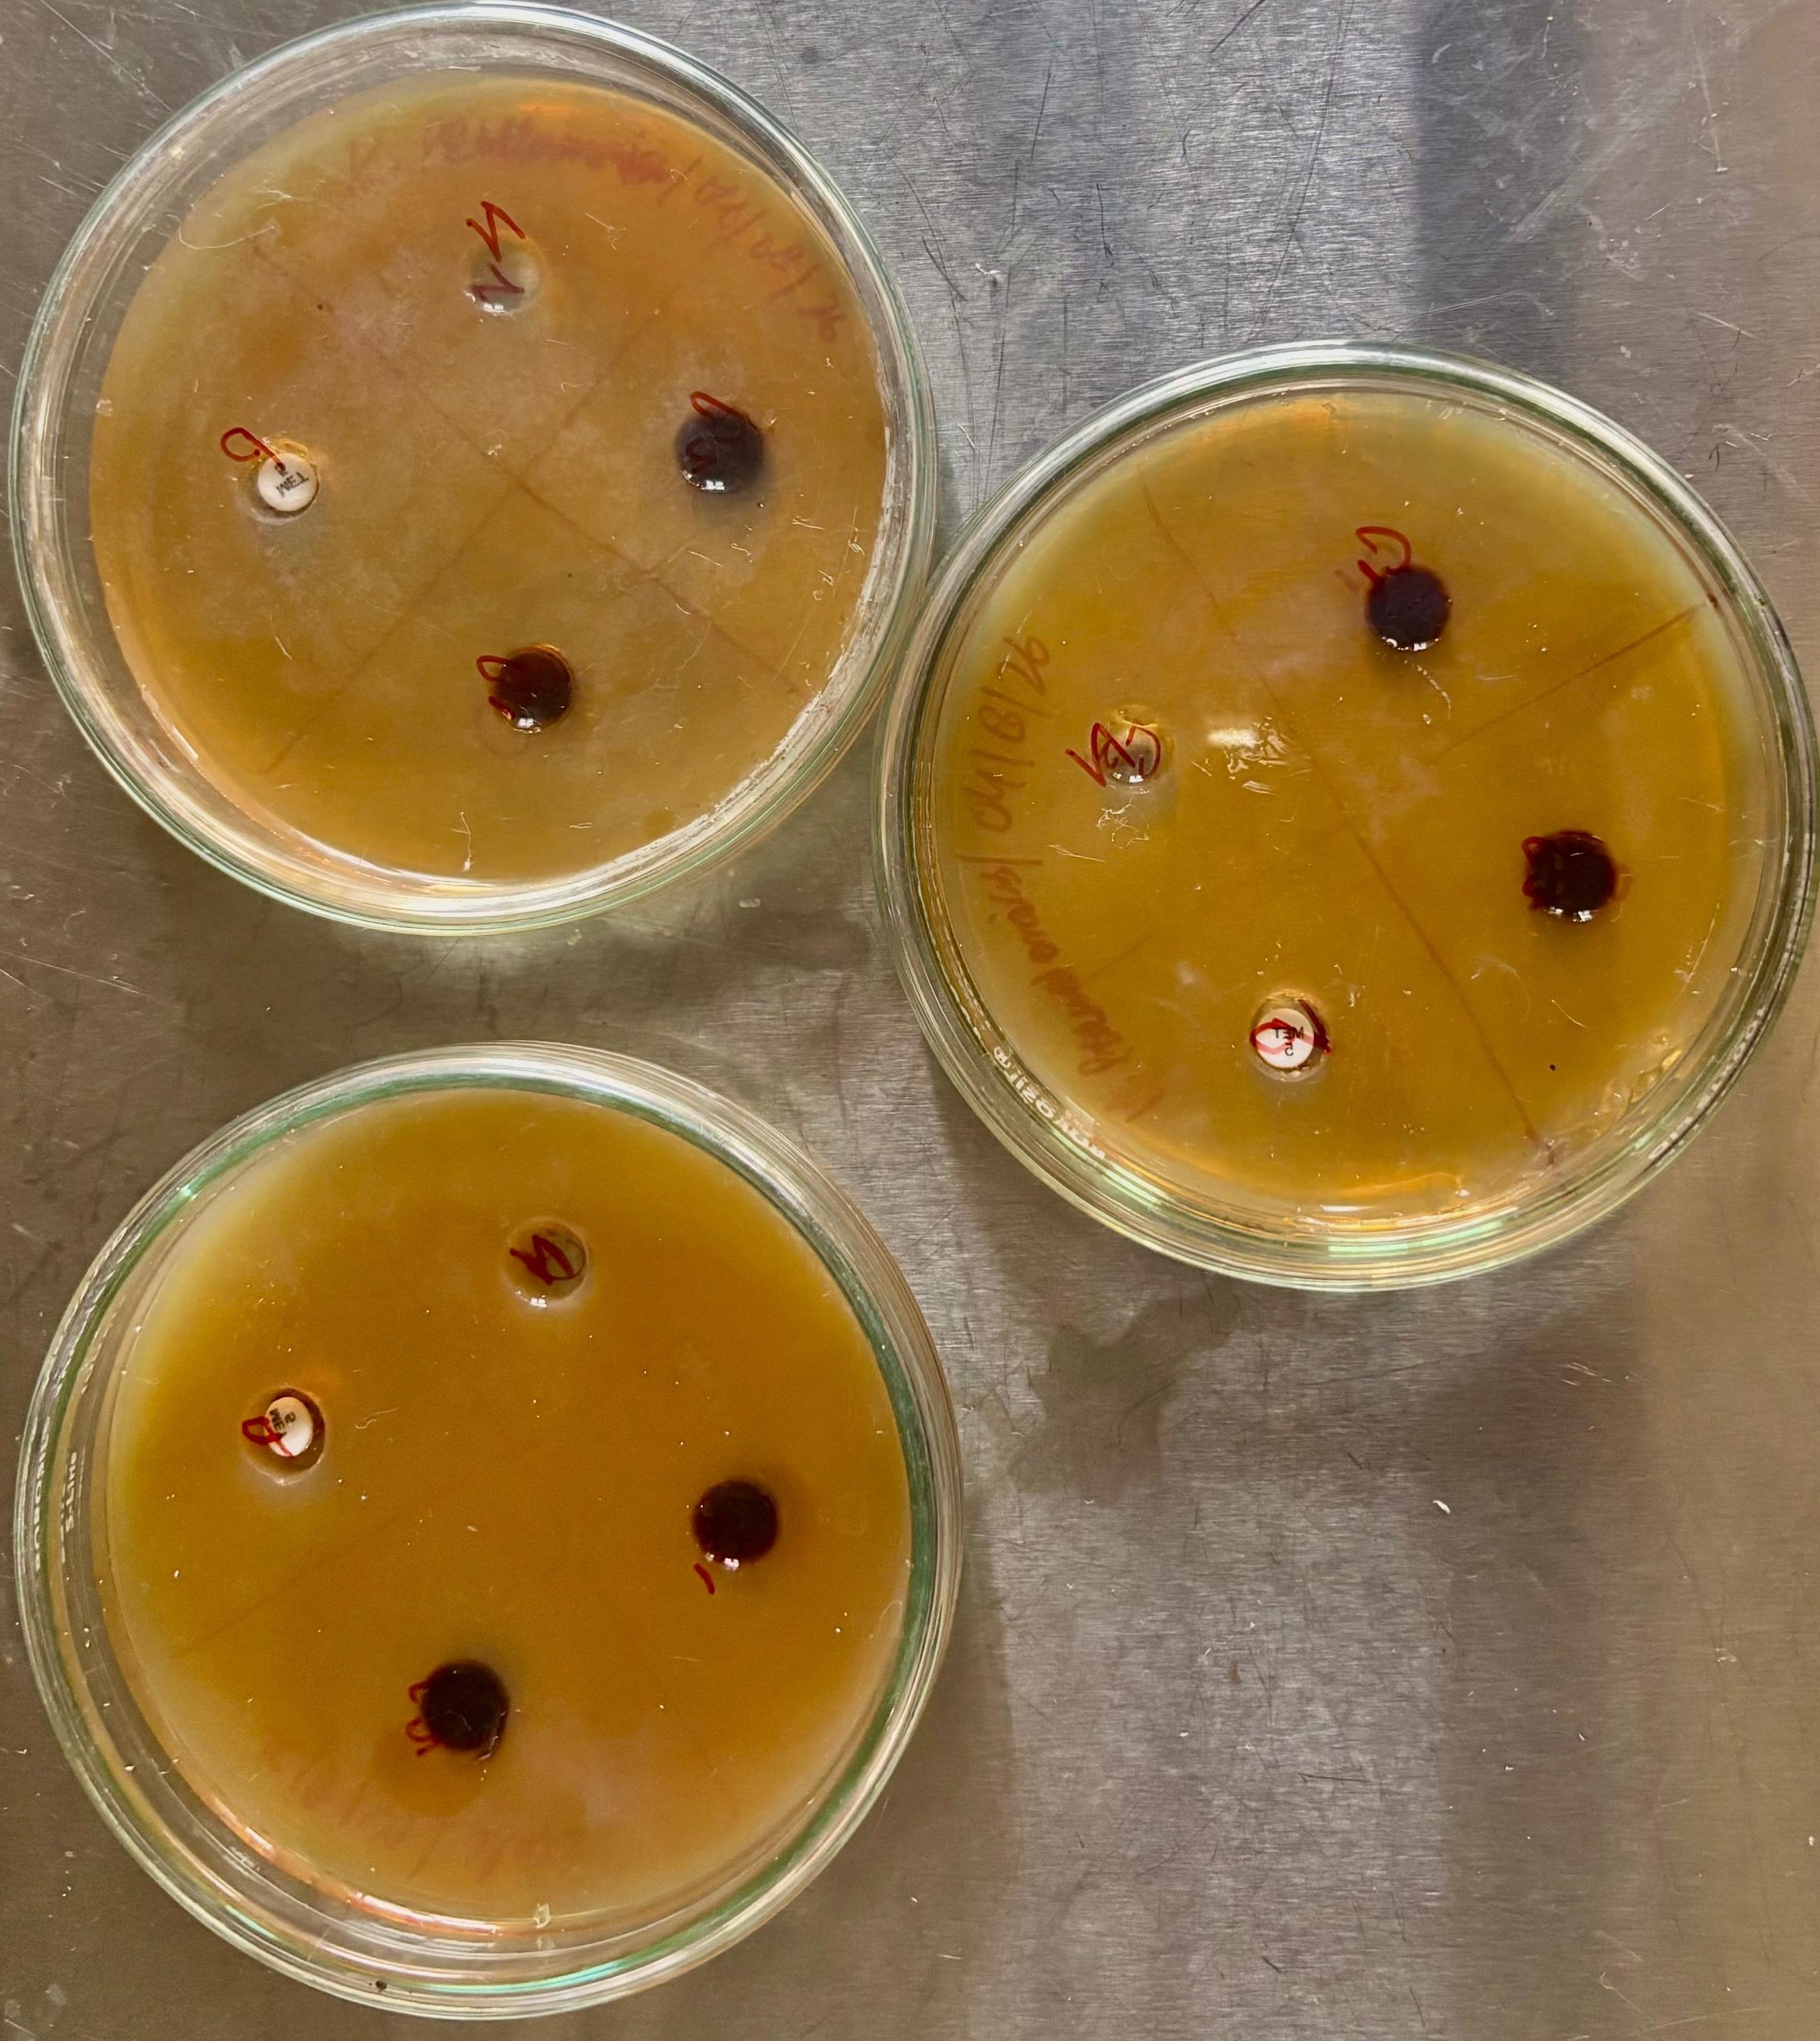
\includegraphics[width=0.88\textwidth]{fig9_assay_trio_dated.jpg}
\caption{Assay plates, 04 August 2026. The upper-left lid reads \textit{K.\ pneumoniae}. The right lid reads Pseudomonas. The species line on the lower plate is not fully legible and is not assigned here. Positions C1, C2, N, and a paper disc are present on each plate.}
\label{fig:assaytrio}
\end{figure}

\begin{figure}[htbp]
\centering
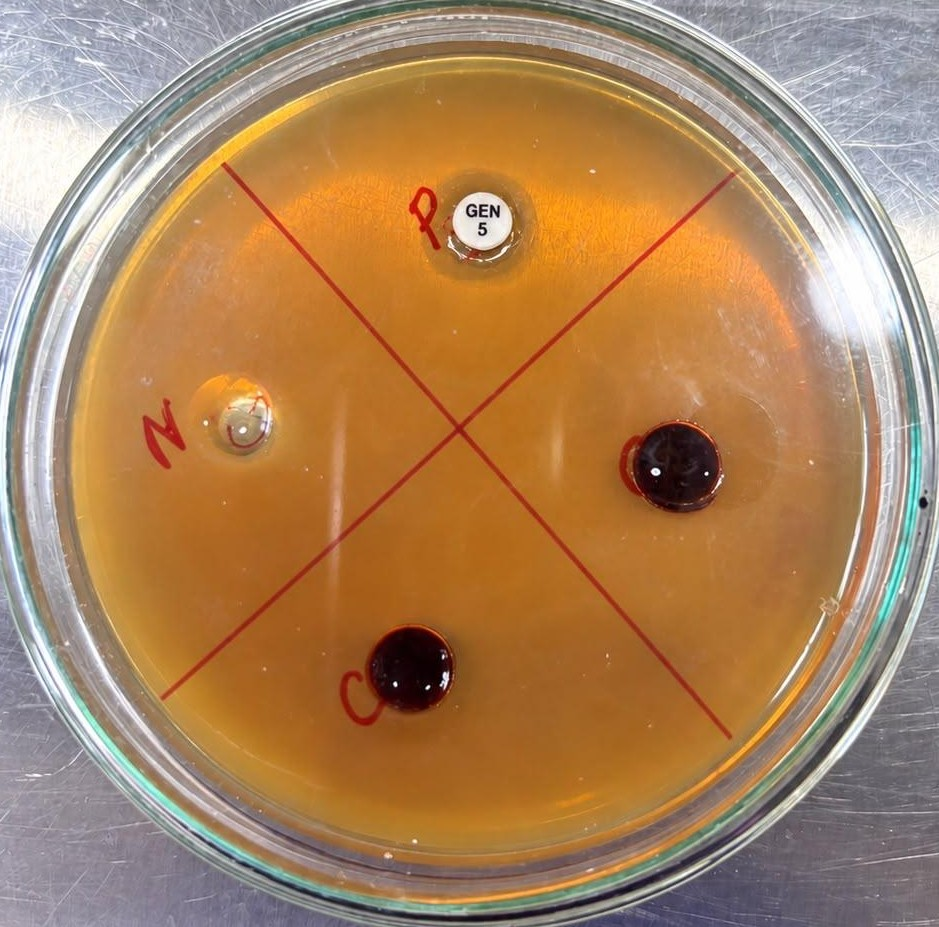
\includegraphics[width=0.62\textwidth]{fig10_gen5_plate.jpg}
\caption{Representative plate showing gentamicin GEN 5 (P), sterile water (N) with no halo, and two extract positions with surrounding clearance. No binomial is written on this close-up.}
\label{fig:gen5}
\end{figure}

\begin{figure}[htbp]
\centering
\begin{tikzpicture}
\begin{axis}[
  ybar,
  bar width=7pt,
  ylabel={Zone of inhibition (mm)},
  ymin=0,
  ymax=22,
  width={0.98\textwidth},
  height=8.2cm,
  enlarge x limits=0.18,
  symbolic x coords={Ecoli, Paer, Kpneu},
  xtick=data,
  xticklabels={\textit{E.\ coli}, \textit{P.\ aeruginosa}, \textit{K.\ pneumoniae}},
  legend style={at={(0.5,-0.22)}, anchor=north, legend columns=3, font=\small, draw=none},
  grid=major,
  grid style={dashed, gray!30},
  /pgf/number format/fixed,
  error bars/y dir=both,
  error bars/y explicit,
]
\addplot+[fill=dissertationblue!70, draw=black, error bars/.cd, y dir=both, y explicit]
  coordinates {(Ecoli,11.94) +-(0.14,0.14) (Paer,16.03) +-(0.25,0.25) (Kpneu,12.35) +-(0.56,0.56)};
\addplot+[fill=dissertationgreen!70, draw=black, error bars/.cd, y dir=both, y explicit]
  coordinates {(Ecoli,14.99) +-(0.51,0.51) (Paer,12.53) +-(0.45,0.45) (Kpneu,13.25) +-(0.43,0.43)};
\addplot+[fill=dissertationgray!50, draw=black, error bars/.cd, y dir=both, y explicit]
  coordinates {(Ecoli,17.00) +-(0.00,0.00) (Paer,17.17) +-(0.29,0.29) (Kpneu,15.17) +-(0.29,0.29)};
\legend{C1 (50 mg/mL), C2 (100 mg/mL), GEN 5}
\end{axis}
\end{tikzpicture}
\caption{Clustered bar graph of mean zone of inhibition ($\pm$ SD) for C1 (\SI{50}{\milli\gram\per\milli\litre}), C2 (\SI{100}{\milli\gram\per\milli\litre}), and gentamicin GEN 5 against the three isolates.}
\label{fig:zoibars}
\end{figure}

Raw triplicate readings are listed in \cref{app:zoi}.

\FloatBarrier

% =========================================================================
% Chapter 5: Discussion
% =========================================================================

\chapter{Discussion}\label{ch:discussion}

The aqueous extract contained the polar classes expected from a water Soxhlet: flavonoids, phenols, tannins, saponins, alkaloids, terpenoids, phytosterols, carbohydrates, and quinones (\cref{tab:phytochem}, \cref{fig:phytochem}). Cowan's catalogue assigns membrane leakage to phenolics and flavonoids, protein binding to tannins, and pore-like disruption to saponins \citep{cowan1999plant,jubair2021review}. Those assignments are consistent with a clear zone around the extract. They are not proof that any one class caused the zone.

Distilled water produced no zone. The solvent therefore does not explain the clearance. GEN 5 produced the widest mean zone on every isolate, as expected for a defined aminoglycoside disc \citep{clsi2024m100}. The extract never matched that disc. C1 and C2 are milligrams per millilitre of a crude concentrate. GEN 5 is five micrograms of a single drug. The comparison is a benchmark, not a potency ratio.

\section{Isolate profiles}

\taxa{Escherichia coli} showed a larger mean zone at C2 than at C1 ($14.99$\,mm versus $11.94$\,mm). That direction matches a simple concentration effect: more solute at C2, more diffusion into the lawn. The outer membrane of \taxa{E. coli} is a barrier \citep{nikaido2003molecular,pages2008porin}, but it did not abolish activity at either strength.

\taxa{Klebsiella pneumoniae} also increased from C1 to C2, but only by about one millimetre ($12.35$\,mm to $13.25$\,mm). The capsule and a typical enterobacterial envelope are a plausible reason for the smaller step \citep{who2024bacterial}. \citet{drakhshaan2026identification} did not test this species, so the values cannot be stacked against their dichloromethane table. They are a new row for the aqueous extract, not a claim of first discovery in the whole \textit{Dipsacus} literature.

\taxa{Pseudomonas aeruginosa} did not follow the same direction. C1 gave $16.03 \pm 0.25$\,mm, the largest extract mean in the study. C2 gave $12.53 \pm 0.45$\,mm, representing an inverted response of $-3.50$\,mm. Calling this isolate ``resistant'' would contradict the C1 plate, where the extract produced a clear, reproducible zone across all three replicates ($16.00$, $16.30$, and $15.80$\,mm; \cref{tab:raw_paer}). Technical explanations, including well-loading discrepancies, pigment masking of the C2 perimeter, or inter-plate agar variation, cannot be excluded. Two biological and physical hypotheses reconcile this non-linear behaviour.

The first hypothesis concerns active efflux kinetics and outer-membrane permeation dynamics. \taxa{Pseudomonas aeruginosa} possesses an envelope with inherently low permeability, governed by the slow porin OprF, in which over 95\% of molecules adopt a closed two-domain conformer with minimal conductance, leaving only 1--5\% in an open $\beta$-barrel conformation \citep{chevalier2017porins}. Active drug extrusion is driven by the tripartite MexAB-OprM efflux pump, in which the inner-membrane proton antiporter MexB operates with the periplasmic adaptor MexA and the outer-membrane duct OprM to expel diverse amphiphilic and aromatic substrates \citep{li1995role,masuda2000substrate}. At C1 (\SI{50}{\milli\gram\per\milli\litre}), passive influx of polar phytochemicals across open OprF channels and surfactant-destabilised lipid domains exceeds basal MexAB-OprM extrusion velocity. Periplasmic and intracellular accumulation reaches inhibitory concentrations, driving cell lysis and establishing a wide clear zone ($16.03$\,mm). At C2 (\SI{100}{\milli\gram\per\milli\litre}), elevated solute influx raises the local concentration to the critical threshold required for MexB allosteric cooperativity or stress-mediated transcriptional induction of the \textit{mexAB-oprM} operon \citep{li1995role,poole2005efflux}. Accelerated active extrusion through OprM outpaces inward diffusion through closed-conformer OprF channels, lowering steady-state intracellular accumulation below lethal levels at the zone periphery and permitting bacterial growth closer to the well ($12.53$\,mm).

The second hypothesis concerns colloidal micellar self-assembly and hydrogel diffusion impedance. Phytochemical analysis confirmed abundant saponins (froth test) and a high extraction yield of 24.13\% (w/w), consistent with substantial recovery of oleanane bidesmosides such as dipsacoside B and asperosaponin VI \citep{zhao2011phytochemicals,skala2023dipsacus}. Amphiphilic saponins assemble into multimolecular micellar aggregates once their concentration exceeds the Critical Micelle Concentration (CMC). At C1 (\SI{50}{\milli\gram\per\milli\litre}), saponin molecules exist predominantly as unassociated monomers that diffuse through the 1.5\% agar hydrogel network. At C2 (\SI{100}{\milli\gram\per\milli\litre}), the concentration surpasses the CMC, promoting self-assembly into bulky micellar aggregates exceeding 50--100\,kDa with substantially enlarged hydrodynamic radii. These macromolecular assemblies suffer severe steric restriction within the fibrous agar matrix. Retarded diffusion is compounded by the high solution viscosity of the concentrated extract, which contains water-soluble polysaccharides and mucilage (evidenced by a strong positive Fehling's reaction; \cref{tab:phytochem}). The resulting steep, truncated diffusion gradient confines the effective inhibitory concentration to a narrower radius around the C2 well.

These interpretations remain reasoned biophysical hypotheses. In the absence of isogenic knockout strains ($\Delta$\textit{mexB}, $\Delta$\textit{oprF}), efflux pump inhibitor controls, or quantitative LC-MS profiling of the specific extract batch, the relative contributions of active efflux induction, micellar aggregation, and technical factors cannot be definitively resolved from agar diffusion assays alone. Candidate metadata limitations noted in earlier chapters---the unrecorded herbarium voucher accession number, lack of ATCC strain accession identifiers, unrecorded extract well loading volume, and unrecorded collection month---prevent direct kinetic modeling. The data are therefore reported as measured, without forcing the numbers into a monotonic concentration gradient.

\section{Comparison with organic-solvent extracts}

\citet{drakhshaan2026identification} used \SI{50}{\micro\gram\per\milli\litre} and \SI{100}{\micro\gram\per\milli\litre} dichloromethane and methanol extracts. Their gentamicin disc was \SI{10}{\micro\gram}. The present C1 and C2 are milligrams per millilitre, a thousand-fold difference on the label, and GEN 5 is not a ten-microgram disc. Millimetre values from that paper are therefore listed only to show that organic extracts of the same species can clear \taxa{E. coli} and \taxa{P. aeruginosa} lawns (\cref{tab:compare}). They are not same-dose replicates.

\begin{table}[htbp]
\centering
\caption{Published zones for organic extracts of \taxa{D.\ inermis} \citep{drakhshaan2026identification} beside the present aqueous means. Units of the extract dose are not the same.}
\label{tab:compare}
\small
\begin{tabular}{@{}>{\raggedright\arraybackslash}p{0.44\textwidth}*{2}{S[table-format=2.2(2)]}@{}}
\toprule
Treatment & {\textit{E.\ coli} (mm)} & {\textit{P.\ aeruginosa} (mm)} \\
\midrule
Present aqueous C2, \SI{100}{\milli\gram\per\milli\litre} & 14.99 \pm 0.51 & 12.53 \pm 0.45 \\
Present aqueous C1, \SI{50}{\milli\gram\per\milli\litre} & 11.94 \pm 0.14 & 16.03 \pm 0.25 \\
DCM \SI{100}{\micro\gram\per\milli\litre} & 15.93 \pm 0.11 & 16.83 \pm 0.29 \\
DCM \SI{50}{\micro\gram\per\milli\litre} & 12.93 \pm 0.11 & 13.10 \pm 0.17 \\
MeOH \SI{100}{\micro\gram\per\milli\litre} & 15.80 \pm 0.34 & 15.17 \pm 0.29 \\
MeOH \SI{50}{\micro\gram\per\milli\litre} & 11.13 \pm 0.23 & 9.07 \pm 0.11 \\
Gentamicin \SI{10}{\micro\gram} (that study) & 15.00 \pm 0.12 & 14.50 \pm 0.30 \\
GEN 5 (this study) & 17.00 \pm 0.00 & 17.17 \pm 0.29 \\
\bottomrule
\end{tabular}
\end{table}

The 24.13\% aqueous yield is much higher than the 2.72\% dichloromethane and 2.9\% methanol yields reported by \citet{drakhshaan2026identification}. Water also extracts sugars, mucilage, and other bulk polar matter as well as phenolics. A high yield does not mean a high titre of antibacterial molecules.

\section{Regional context}

Kashmiri use of wopal haakh as a boiled leaf preparation \citep{lone2015study,haq2023cross,ahad2023ethnobotanical} is an aqueous tradition. The Soxhlet water extract is a laboratory relative of that solvent, not a clinical decoction trial. The NF-$\kappa$B study from the same university shows that local \taxa{D. inermis} is pharmacologically active \citep{hassan2020dipsacus}. Antibacterial zones on LB plates do not extend that claim to patients.

\section{Limits}

The screen used two concentrations, one solvent, three isolates without accession numbers, LB rather than Mueller--Hinton agar, and zone of inhibition only. MIC and MBC were not measured. GC-MS and LC-MS of the aqueous concentrate were not done. Some plates in the photograph set carry MET 5 discs; those discs were not entered in \cref{tab:zoi}. Collection month and a herbarium voucher number were not available. The work is a preliminary \invitro{} record for an aqueous extract from the Botanical Garden stand.

\FloatBarrier

% =========================================================================
% Chapter 6: Conclusion and Future Prospects
% =========================================================================

\chapter{Conclusion and Future Prospects}\label{ch:conclusion}

The three objectives were met within the limits of a zone-of-inhibition screen.

Plant material of \taxa{Dipsacus inermis} was collected from the Kashmir University Botanical Garden at 34.12981$^{\circ}$\,N, 74.83396$^{\circ}$\,E (WGS84), authenticated at the Centre for Biodiversity and Taxonomy, dried, powdered, and extracted with distilled water in a Soxhlet apparatus. The concentrate was reconstituted at \SI{50}{\milli\gram\per\milli\litre} (C1) and \SI{100}{\milli\gram\per\milli\litre} (C2).

Qualitative tubes were positive for alkaloids, flavonoids, phenols, tannins, saponins, terpenoids, phytosterols, carbohydrates, and quinones.

Both extract concentrations produced zones against \taxa{Escherichia coli}, \taxa{Pseudomonas aeruginosa}, and \taxa{Klebsiella pneumoniae} held in the Advanced Research Laboratory. Distilled water produced none. GEN 5 remained the widest reference. Zones were measured inclusive of the disc. \taxa{E. coli} and \taxa{K. pneumoniae} gave larger means at C2 than at C1. \taxa{P. aeruginosa} gave its largest extract mean at C1. The aqueous extract is therefore active \invitro{} on these lawns, but activity is not a simple function of the two labelled strengths, and it is not a clinical result.

Future work should determine MIC and MBC in broth, preferably on Mueller--Hinton medium with identified strains. LC-MS or GC-MS of the aqueous concentrate would show which polar peaks are present. A wider concentration series would test whether the \taxa{P. aeruginosa} inversion repeats. Until those data exist, the present tables should be read as a preliminary aqueous screen of a Kashmir Botanical Garden collection, not as a treatment claim.

\FloatBarrier


\clearpage
\phantomsection
\addcontentsline{toc}{chapter}{References}
\printbibliography[title={REFERENCES}]

\appendix
% =========================================================================
% Appendix A: Raw triplicate ZOI readings
% =========================================================================

\chapter{Raw zone-of-inhibition replicates}\label{app:zoi}

Triplicate millimetre readings from which \cref{tab:zoi} was calculated. Zones were measured inclusive of the disc. C1 = \SI{50}{\milli\gram\per\milli\litre}; C2 = \SI{100}{\milli\gram\per\milli\litre}; GEN 5 = gentamicin \SI{5}{\micro\gram} disc; N = distilled water.

\begin{table}[htbp]
\centering
\caption{Raw zone diameters (mm) for \taxa{Escherichia coli}.}
\label{tab:raw_ecoli}
\begin{tabular}{@{}l*{3}{S[table-format=2.2]}@{}}
\toprule
Treatment & {R1} & {R2} & {R3} \\
\midrule
C1 & 12.00 & 11.78 & 12.05 \\
C2 & 15.00 & 15.50 & 14.48 \\
GEN 5 & 17.00 & 17.00 & 17.00 \\
N & 0.00 & 0.00 & 0.00 \\
\bottomrule
\end{tabular}
\end{table}

\begin{table}[htbp]
\centering
\caption{Raw zone diameters (mm) for \taxa{Pseudomonas aeruginosa}.}
\label{tab:raw_paer}
\begin{tabular}{@{}l*{3}{S[table-format=2.2]}@{}}
\toprule
Treatment & {R1} & {R2} & {R3} \\
\midrule
C1 & 16.00 & 16.30 & 15.80 \\
C2 & 13.00 & 12.50 & 12.10 \\
GEN 5 & 17.50 & 17.00 & 17.00 \\
N & 0.00 & 0.00 & 0.00 \\
\bottomrule
\end{tabular}
\end{table}

\begin{table}[htbp]
\centering
\caption{Raw zone diameters (mm) for \taxa{Klebsiella pneumoniae}.}
\label{tab:raw_kpneu}
\begin{tabular}{@{}l*{3}{S[table-format=2.2]}@{}}
\toprule
Treatment & {R1} & {R2} & {R3} \\
\midrule
C1 & 12.00 & 13.00 & 12.05 \\
C2 & 13.50 & 13.50 & 12.75 \\
GEN 5 & 15.50 & 15.00 & 15.00 \\
N & 0.00 & 0.00 & 0.00 \\
\bottomrule
\end{tabular}
\end{table}


\end{document}
